%~~~~~~~~~~~~~~~~~~~~~~~~~~~~~~~~~~~~~~~~~~~~~~~~~~~~~~~~~~~~~~~~~~~~~
%    File      : webanalysis
%~~~~~~~~~~~~~~~~~~~~~~~~~~~~~~~~~~~~~~~~~~~~~~~~~~~~~~~~~~~~~~~~~~~~~

\textual

%\chapter{Dependability}\label{cap:dependability}

\section{Documentazione Server Tomcat}

In questa sezione vengono mostrati i diagrammi UML relativamente alla realizzazione del Server Tomcat, su cui sono installate le Servlet per la gestione delle politiche di login e registrazione, nonché l'interfacciamento con la base di dati e con il mail server.

\subsection{Diagramma delle Classi}

Di seguito viene riportato il diagramma delle classi di Secure Messaging: piuttosto che limitarci ad allegare un solo diagramma, troppo complesso e poco informativo, si riportano le classi per package e relazioni intra ed inter-package; in questo modo abbiamo suddiviso il diagramma delle classi originali in porzioni sufficientemente piccole da poter essere analizzate con profitto ma sufficientemente grandi da essere significative, che nell’insieme permette ad un programmatore la giusta documentazione per individuare struttura e dipendenza delle classi con l’adeguata granularità di informazioni.
Per ragioni di semplicità sono state omesse le relazioni al package delle eccezioni, da cui praticamente tutti i package dipendono.

\subsubsection{Package: \textbf{access control}}

Contiene la classe che si occupa delle operazioni per prevenire o individuare le intrusioni in un account, aggiornare i conteggi dei login falliti e bloccare i tentativi di accesso.

\begin{figure}[!htbp]
	\centering
	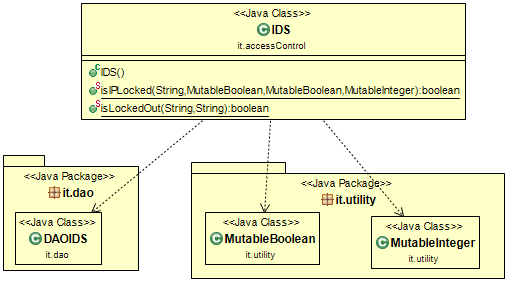
\includegraphics[scale = .6]{img/dependencies_accesscontrol.png}
	\caption{Package Access Control}
	\label{gfx:accesscontrol}
\end{figure}


\subsubsection{Package: \textbf{authentication}}

Appartengono a questo package la servlet di autenticazione e la relativa logica (disaccoppiata dalla servlet per il principio della separazione degli interessi). Il package è visualizzato in figura \ref{gfx:dependencies_authentication}.

\tiny 
\begin{landscape}
\begin{center}
\vspace*{\fill}
\begin{figure}[!htbp]
	\centering
	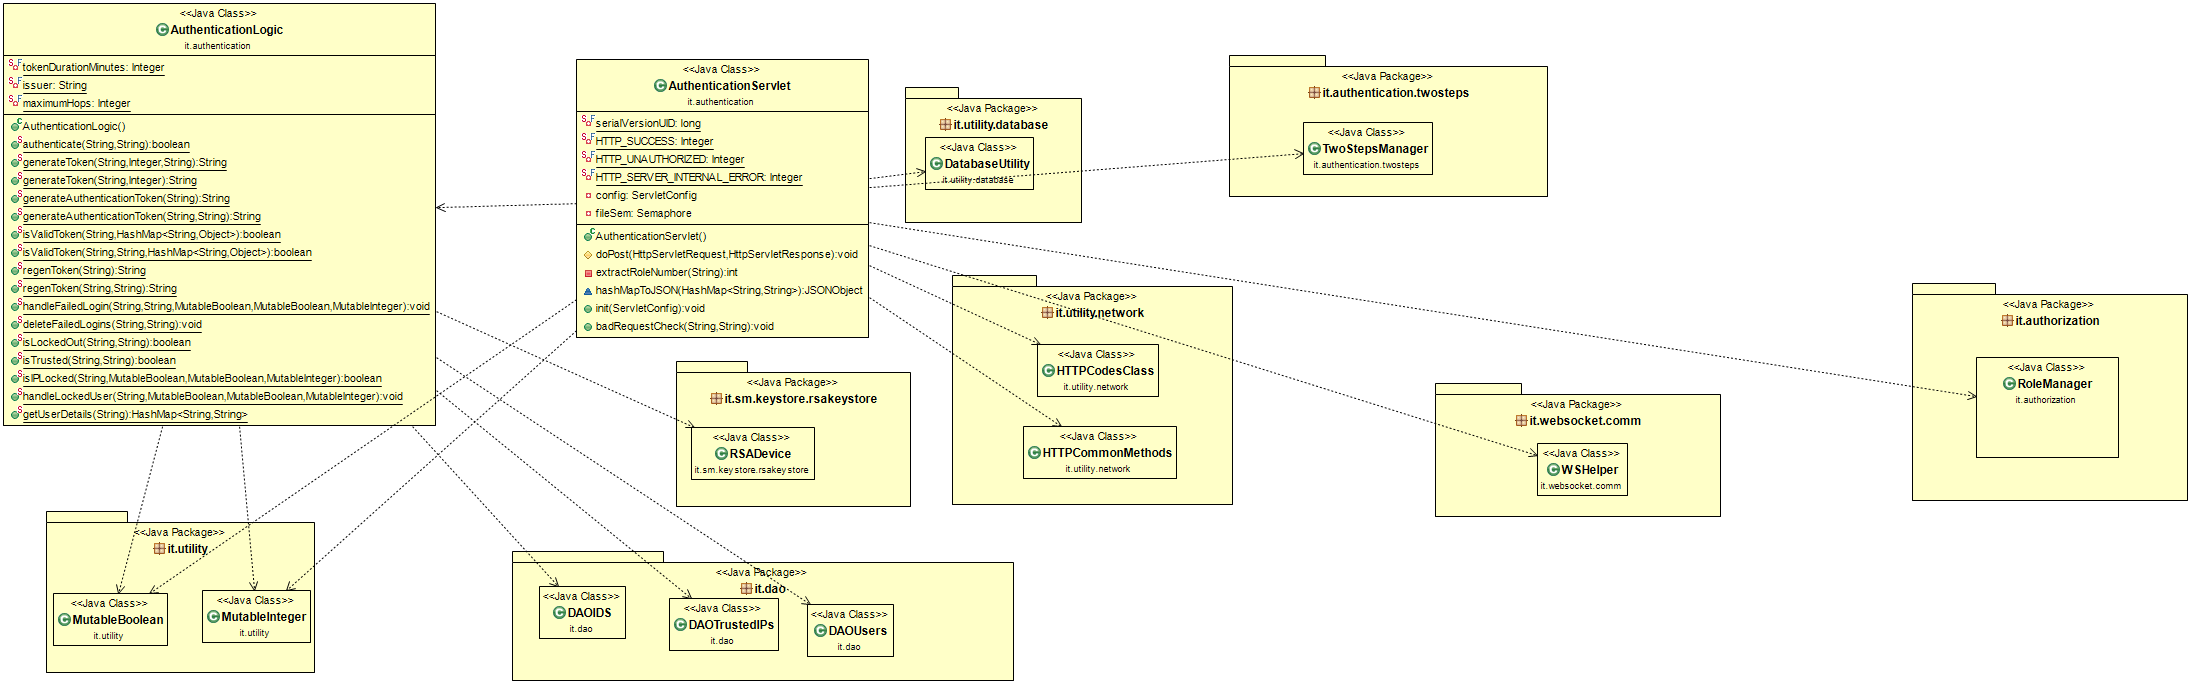
\includegraphics[scale = .3]{img/dependencies_authentication}
	\caption{Package Authentication}
	\label{gfx:dependencies_authentication}
\end{figure}
\vspace*{\fill}

\end{center}	

\end{landscape}%
\normalsize

\subsubsection{Package: \textbf{authorization}}

Le classi di questo package si occupano di determinare se l’utente è autorizzato ad effettuare una determinata operazione.\\
In particolare, contiene un filtro (ContactListFilter) che si occupa di filtrare le richieste che vengono fatte verso le diverse contact-lists disponibili, ed accettarle in base al rispetto delle policy XACML previste.

Il package è visualizzato in figura \ref{gfx:dependencies_authorization}.

\begin{figure}[!htbp]
	\centering
	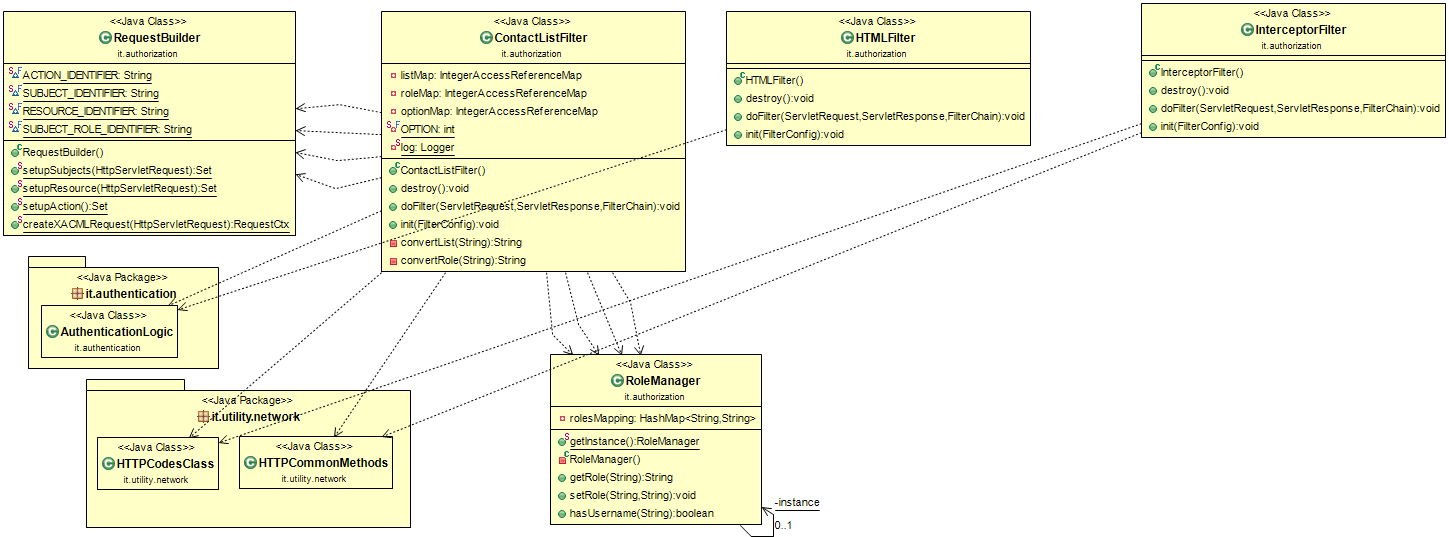
\includegraphics[scale = .3]{img/dependencies_authorization}
	\caption{Package Authorization}
	\label{gfx:dependencies_authorization}
\end{figure}

\subsubsection{Package: \textbf{bcrypt}}

Package importato da una libreria OTS che implementa hashing/salting delle password con algoritmo bcrypt (utilizzato, fra gli altri, da OpenBSD). 
Il package è visualizzato in figura \ref{gfx:dependencies_bcrypt}.

\begin{figure}[!htbp]
	\centering
	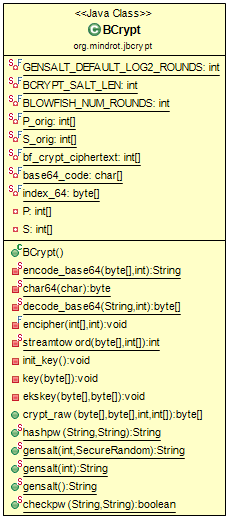
\includegraphics[scale = .5]{img/dependencies_bcrypt}
	\caption{Package BCrypt}
	\label{gfx:dependencies_bcrypt}
\end{figure}

\subsubsection{Package: \textbf{DAO}}

Questo package rappresenta il ponte tra i dati del database e l’applicazione. Sono le classi a cui le altre si rivolgono per operare su dati che altrimenti sarebbero da prelevare direttamente dal database. 

Il package è visualizzato in figura \ref{gfx:dependencies_dao}.

\begin{figure}[!htbp]
	\centering
	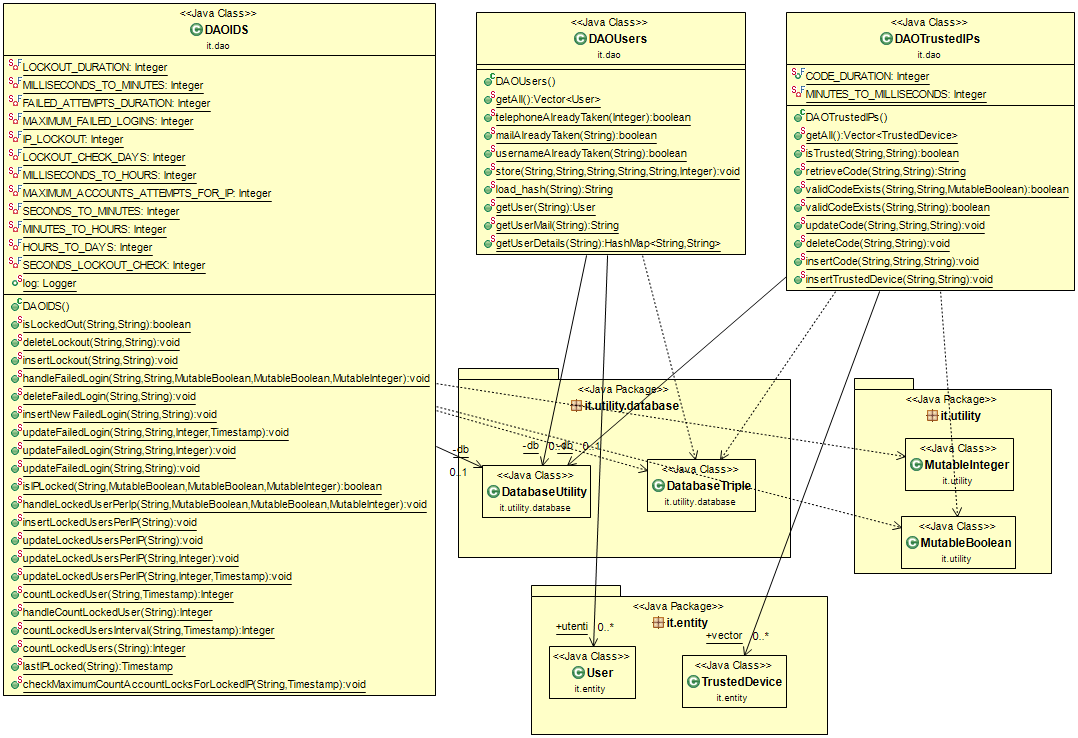
\includegraphics[scale = .4]{img/dependencies_dao}
	\caption{Package DAO}
	\label{gfx:dependencies_dao}
\end{figure}

\subsubsection{Package: \textbf{entity}}

Costituiscono una rappresentazione Object-oriented che effettua il mapping rispetto alla rappresentazione del db.

Il package è visualizzato in figura \ref{gfx:dependencies_entity}.

\begin{figure}[!htbp]
	\centering
	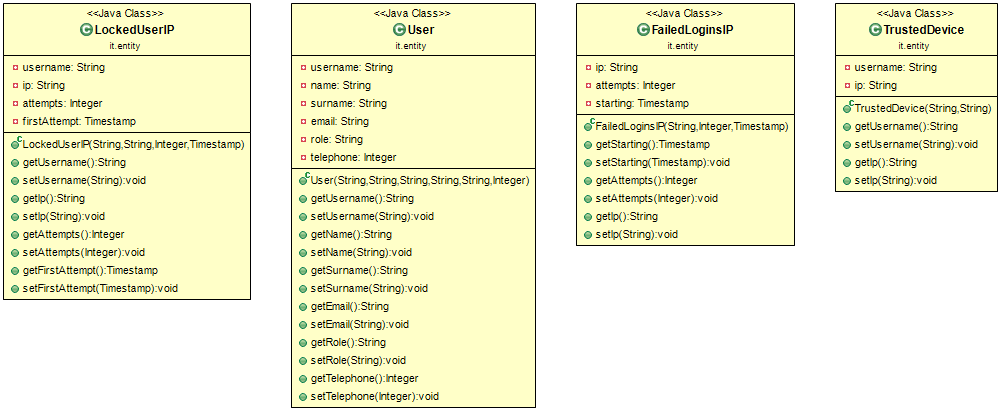
\includegraphics[scale = .4]{img/dependencies_entity}
	\caption{Package Entity}
	\label{gfx:dependencies_entity}
\end{figure}

\subsubsection{Package: \textbf{exception}}

Raccoglie tutte le eccezioni che possono essere lanciate. A sua volta è diviso in sotto-package che non vengono rappresentati per semplicità.

Il package è visualizzato in figura \ref{gfx:dependencies_exception}, a pagina successiva.

\tiny 
\begin{landscape}
\begin{center}
\vspace*{\fill}
\begin{figure}[!htbp]
	\centering
	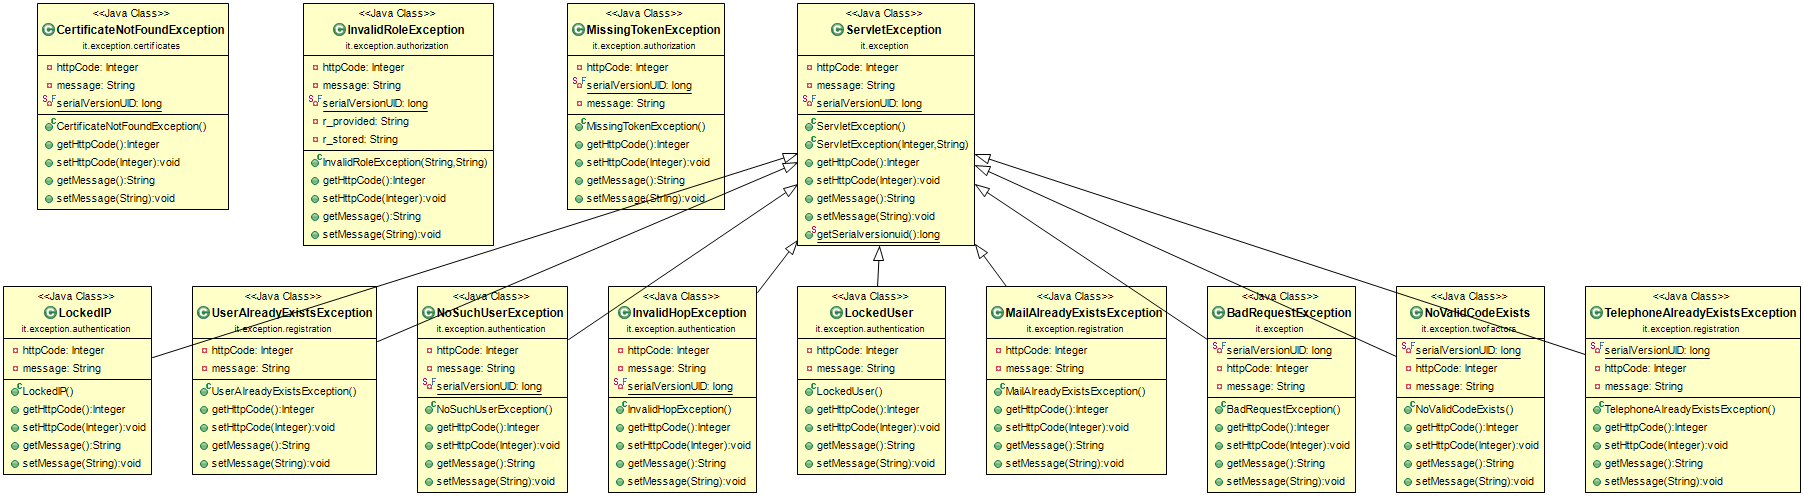
\includegraphics[scale = .3]{img/dependencies_exception}
	\caption{Package Exception}
	\label{gfx:dependencies_exception}
\end{figure}
\vspace*{\fill}

\end{center}	

\end{landscape}%
\normalsize
\subsubsection{Package: \textbf{keystore}}

Contiene la semplice interfaccia che ci aspetteremmo da un’entità crittografica: la capacità di criptare e decriptare bytes. Implementeranno l’interfaccia tutte quelle classi che si occuperanno di crittografare dati (implementando gli specifici algoritmi di cui MyKeystore è indipendente).

Il package è visualizzato in figura \ref{gfx:dependencies_keystore}.

\begin{figure}[!htbp]
	\centering
	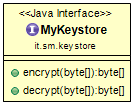
\includegraphics[scale = .5]{img/dependencies_keystore}
	\caption{Package Keystore}
	\label{gfx:dependencies_keystore}
\end{figure}

\subsubsection{Package: \textbf{keystore.rsaKeystore}}

Package innestato nel precedente che rappresenta una crittografia specifica, in questo caso di tipo RSA. Simula le caratteristiche di una smart-card (di cui avremmo bisogno per una criptografia sicura) in software, e usa le chiavi private e pubblica per codificare e decodificare: la privata viene usate per codificare i dati da mandare al client, la pubblica quelli che solo il server può leggere, come la chiave AES utilizzata per codificare i parametri di accesso al db e al mail server.


Il package è visualizzato in figura \ref{gfx:keystore.rsaKeystore}.

\begin{figure}[!htbp]
	\centering
	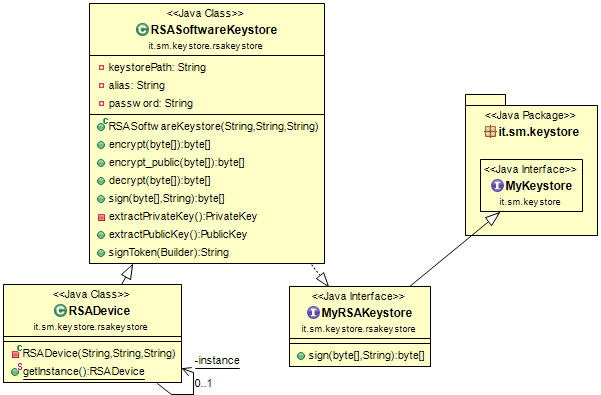
\includegraphics[scale = .5]{img/dependencies_rsakeystore.png}
	\caption{Package keystore.rsaKeystore}
	\label{gfx:keystore.rsaKeystore}
\end{figure}

\subsubsection{Package: \textbf{registration}}

Appartengono a questo package la servlet e la logica di registrazione.


Il package è visualizzato in figura \ref{gfx:registration}.

\begin{figure}[!htbp]
	\centering
	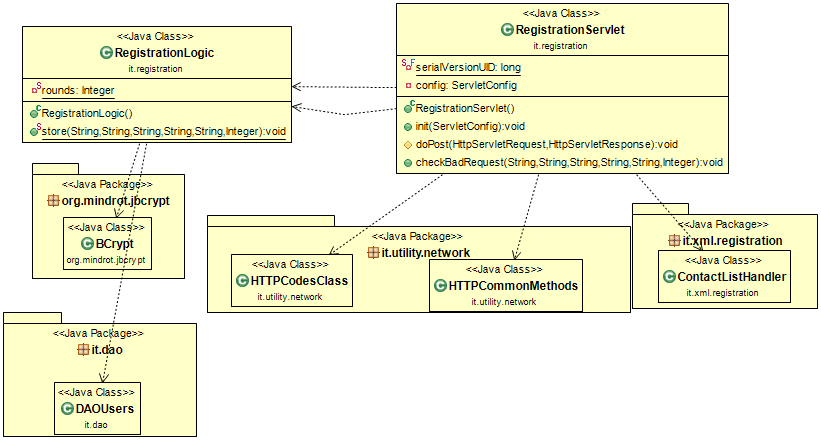
\includegraphics[scale = .5]{img/dependencies_registration.png}
	\caption{Package Registration}
	\label{gfx:registration}
\end{figure}


\subsubsection{Package: \textbf{twosteps}}

Di questo package fanno parte le classi che si occupano dell’autenticazione in due passi; la classe TwoStepsServlet rappresenta la servlet a cui rivolgersi per l’invio del codice, ed effettua chiamate a TwoStepsLogic per ciò che concerne la logica delle operazioni, mentre TwoStepsManager si occupa dell’invio della mail nel caso in cui fosse richiesta.

Il package è visualizzato in figura \ref{gfx:dependencies_twosteps}.

\begin{figure}[!htbp]
	\centering
	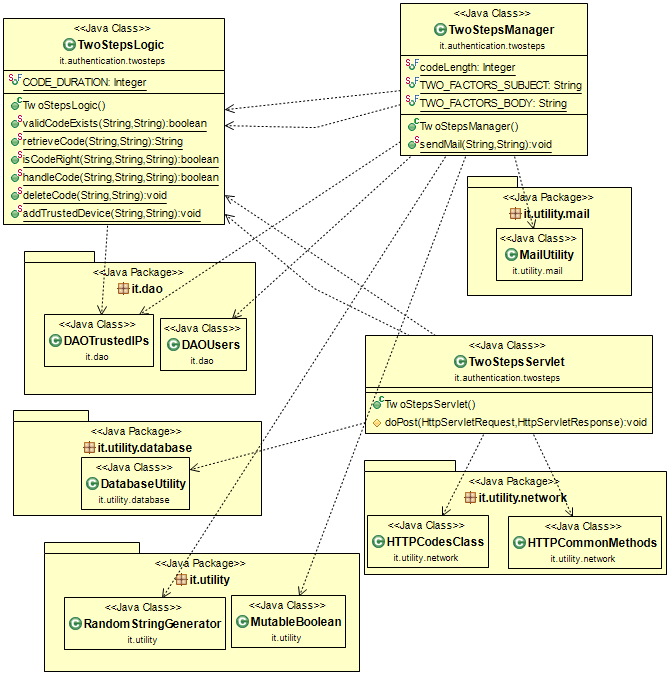
\includegraphics[scale = .5]{img/dependencies_twosteps.png}
	\caption{Package Twosteps}
	\label{gfx:dependencies_twosteps}
\end{figure}

\subsubsection{Package: \textbf{utility}}

Contiene diverse classi di utilità, utilizzate per risolvere in modo semplice alcuni semplici compiti, come la generazione del codice per l’autenticazione a due step (RandomStringGenerator).


Il package è visualizzato in figura \ref{gfx:dependencies_utility}.

\begin{figure}[!htbp]
	\centering
	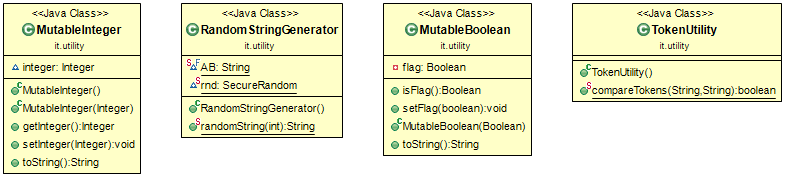
\includegraphics[scale = .5]{img/dependencies_utility}
	\caption{Package Utility}
	\label{gfx:dependencies_utility}
\end{figure}

\subsubsection{Package: \textbf{utility.database}}

A questo package appartengono delle classi di utilità create per rendere più semplice alcune operazioni di routine sul database.

Il package è visualizzato in figura \ref{gfx:dependencies_utilitydatabase}.

\begin{figure}[!htbp]
	\centering
	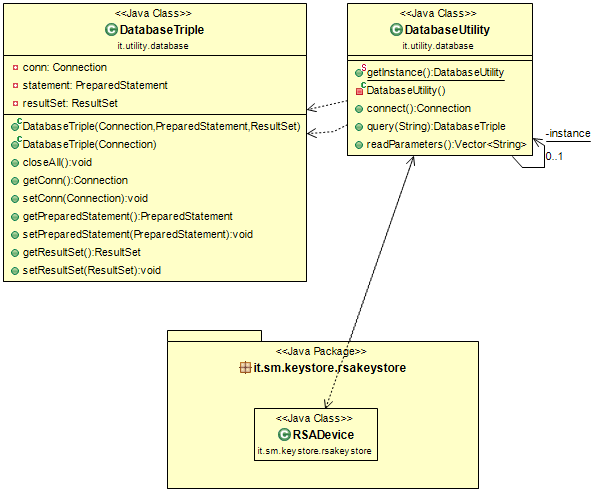
\includegraphics[scale = .5]{img/dependencies_utility_database}
	\caption{Package utility.database}
	\label{gfx:dependencies_utilitydatabase}
\end{figure}

\subsubsection{Package: \textbf{utility.mail}}

Contiene la classe per l’interfacciamento al mail server.

Il package è visualizzato in figura \ref{gfx:dependencies_utilitymail}.

\begin{figure}[!htbp]
	\centering
	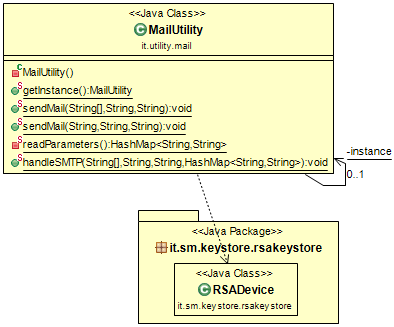
\includegraphics[scale = .5]{img/dependencies_utility_mail}
	\caption{Package utility.mail}
	\label{gfx:dependencies_utilitymail}
\end{figure}

\subsubsection{Package: \textbf{utility.network}}

Contiene la classe per l’interfacciamento al mail server.

Il package è visualizzato in figura \ref{gfx:dependencies_utility_network}.

\begin{figure}[!htbp]
	\centering
	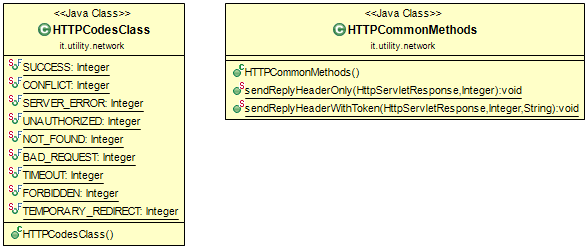
\includegraphics[scale = .5]{img/dependencies_utility_network}
	\caption{Package utility.network}
	\label{gfx:dependencies_utility_network}
\end{figure}

\subsubsection{Package: \textbf{webfilter}}

Le classi di questo package risolvono diversi problemi come il Cross Origin Resource Sharing.
Il package è visualizzato in figura \ref{gfx:dependencies_webfilter}.

\begin{figure}[!htbp]
	\centering
	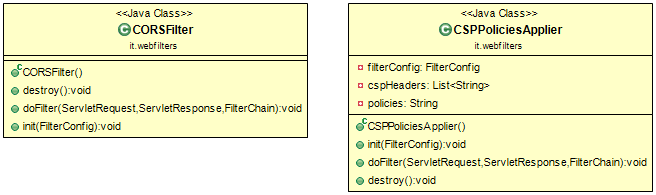
\includegraphics[scale = .5]{img/dependencies_webfilter}
	\caption{Package webfilter}
	\label{gfx:dependencies_webfilter}
\end{figure}


\subsubsection{Package: \textbf{websocket}}

Questo package contiene le classi per la gestione delle Web Socket.
In particolare, contiene classi che consentono l'interfacciamento con il server nodeJS e la comunicazione dei dati relativi agli utenti che hanno correttamente effettuato la procedura di login.\\
Infatti, nel momento in cui un utente effettua il login presso il server principale, le sue informazioni saranno inoltrate anche al server nodeJS: per evitare la falsificazione delle informazioni che vengono inviate al server nodeJS, sono state predisposte alcune misure di sicurezza con cui il server nodeJS è in grado di capire se il messaggio ricevuto proviene effettivamente dal server principale o meno: per ulteriori dettagli, si rimanda ai sequence diagram relativi alla fase di login.\\

Il package è visualizzato in figura \ref{gfx:dependencies_websocket}.

\begin{figure}[!htbp]
	\centering
	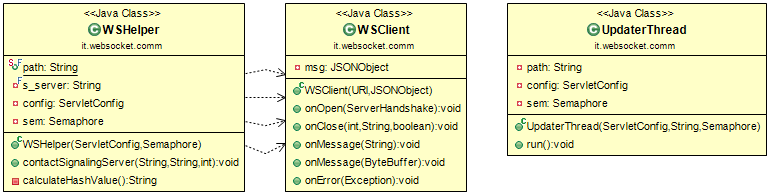
\includegraphics[scale = .5]{img/dependencies_websocket}
	\caption{Package websocket}
	\label{gfx:dependencies_websocket}
\end{figure}

\subsubsection{Package: \textbf{xml.registration}}

Il package è visualizzato in figura \ref{gfx:dependencies_xmlregistration}.

\begin{figure}[!htbp]
	\centering
	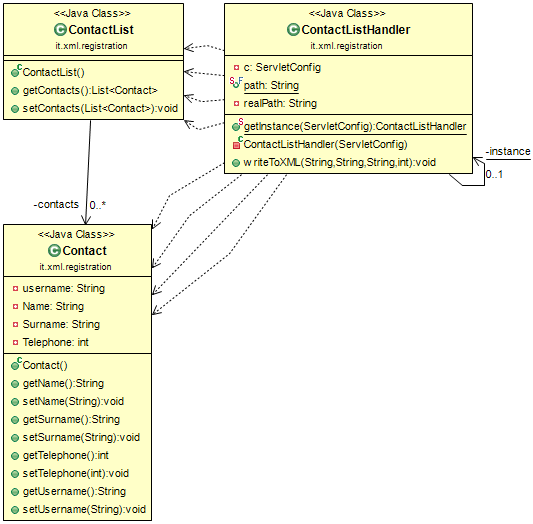
\includegraphics[scale = .5]{img/dependencies_xmlregistration}
	\caption{Package websocket}
	\label{gfx:dependencies_xmlregistration}
\end{figure}